\documentclass[conference]{IEEEtran}

%%%%%%%%%%%%%%%%%%%%%%%%%%%%%%%%%%%%%%%%%%%%%%%%%%%%%%%%%%%%%%%%%%%%%%%%%%%%%%%%%%%%%%%%%%%%%%%%%%%%%%%%%%
\usepackage{amsmath,bm}
\usepackage{graphicx}

\def\MLine#1{\par\hspace*{-\leftmargin}\parbox{\textwidth}{\[#1\]}}
\graphicspath{ {./Images/} }
%%%%%%%%%%%%%%%%%%%%%%%%%%%%%%%%%%%%%%%%%%%%%%%%%%%%%%%%%%%%%%%%%%%%%%%%%%%%%%%%%%%%%%%%%%%%%%%%%%%%%%%%%%

%%%%%%%%%%%%%%%%%%%%%%%%%%%%%%%%%%%%%%%%%%%%%%%%%%%%%%%%%%%%%%%%%%%%%%%%%%%%%%%%%%%%%%%%%%%%%%%%%%%%%%%%%%
\begin{document}
%%%%%%%%%%%%%%%%%%%%%%%%%%%%%%%%%%%%%%%%%%%%%%%%%%%%%%%%%%%%%%%%%%%%%%%%%%%%%%%%%%%%%%%%%%%%%%%%%%%%%%%%%%
\title{Software systems}
\author{Xin Wang}
%%%%%%%%%%%%%%%%%%%%%%%%%%%%%%%%%%%%%%%%%%%%%%%%%%%%%%%%%%%%%%%%%%%%%%%%%%%%%%%%%%%%%%%%%%%%%%%%%%%%%%%%%%
\maketitle
%%%%%%%%%%%%%%%%%%%%%%%%%%%%%%%%%%%%%%%%%%%%%%%%%%%%%%%%%%%%%%%%%%%%%%%%%%%%%%%%%%%%%%%%%%%%%%%%%%%%%%%%%%
\section{Overview}
%%%%%%%%%%%%%%%%%%%%%%%%%%%%%%%%%%%%%%%%%%%%%%%%%%%%%%%%%%%%%%%%%%%%%%%%%%%%%%%%%%%%%%%%%%%%%%%%%%%%%%%%%%
\subsection{Analysing software systems}

\begin{itemize}
    \item Aspects to consider:
    \begin{itemize}
        \item System high-level functions
        \item System nodes
        \item Types of data managed and processed
        \item Data movement within the system
    \end{itemize}

    \item Usually expressed with pictures
\end{itemize}

%%%%%%%%%%%%%%%%%%%%%%%%%%%%%%%%%%%%%%%%%%%%%%%%%%%%%%%%%%%%%%%%%%%%%%%%%%%%%%%%%%%%%%%%%%%%%%%%%%%%%%%%%%
\subsection{Modelling data (Database)}

\begin{itemize}
    \item Data is always stored, transformed and analysed
    \item \textbf{Abstract Data Model} used to understand process
    \item \textbf{Database theory} creates the Abstract Data Model
    \item Database theory considers:
    \begin{itemize}
        \item Important entities in Database
        \item \textbf{Attributes} of these entities
        \item \textbf{Relationships} between these entities
    \end{itemize}
    \item \textbf{Entity modelling} formally expresses database theory
    \item \textbf{Database systems} implements the Abstract Data Model
\end{itemize}

%%%%%%%%%%%%%%%%%%%%%%%%%%%%%%%%%%%%%%%%%%%%%%%%%%%%%%%%%%%%%%%%%%%%%%%%%%%%%%%%%%%%%%%%%%%%%%%%%%%%%%%%%%
\subsection{Moving data (Network)}

\begin{itemize}
    \item Process of data moving between nodes
    \item \textbf{Network models} defines the type of network structure
    \item \textbf{Network protocol} and \textbf{API} implements the model
\end{itemize}

%%%%%%%%%%%%%%%%%%%%%%%%%%%%%%%%%%%%%%%%%%%%%%%%%%%%%%%%%%%%%%%%%%%%%%%%%%%%%%%%%%%%%%%%%%%%%%%%%%%%%%%%%%
\section{Entity Relation Modelling}
%%%%%%%%%%%%%%%%%%%%%%%%%%%%%%%%%%%%%%%%%%%%%%%%%%%%%%%%%%%%%%%%%%%%%%%%%%%%%%%%%%%%%%%%%%%%%%%%%%%%%%%%%%
\begin{itemize}
    \item Creates \textbf{Entity Relationship Diagram}
    \item Establishing \textbf{relationships} in a given system:
    \begin{itemize}
        \item \textbf{Entities}: Aspects within a given system
        \item \textbf{Relationships}: How entities are related
        \item \textbf{Attributes}: Properties of an entity or relationship
    \end{itemize}
    \item Captures constraints and requirements on data 
    \item Used as a guide to \textit{implement} relations
\end{itemize}
\begin{figure} [h!]
    \centering
    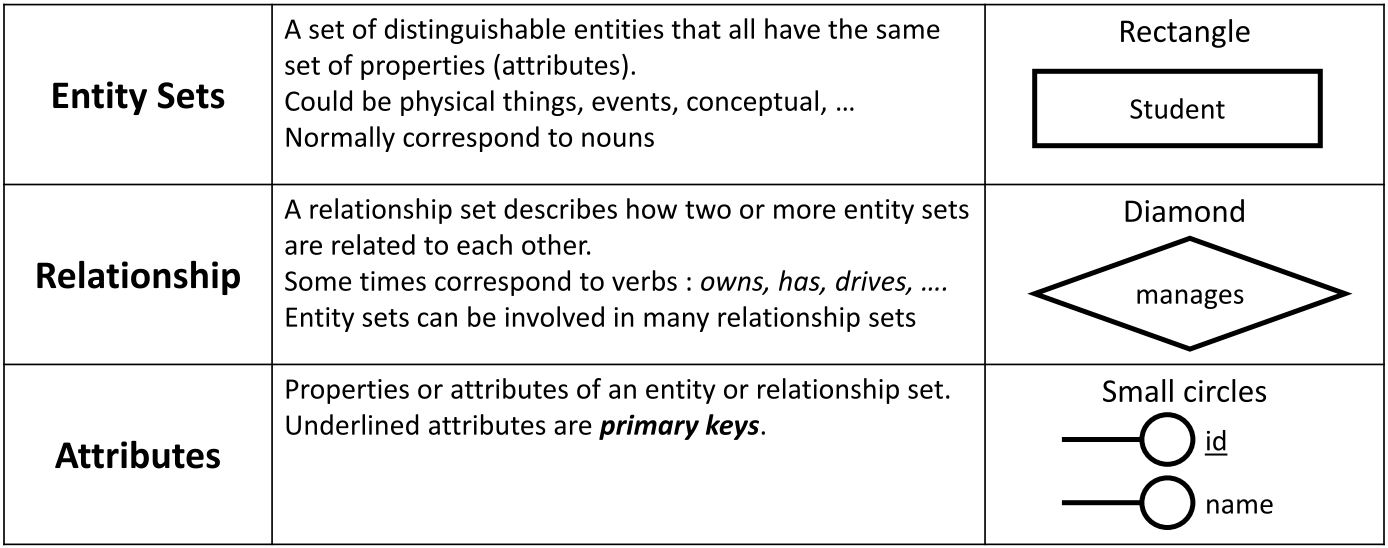
\includegraphics[scale=0.3]{ERM.JPG}
\end{figure}

%%%%%%%%%%%%%%%%%%%%%%%%%%%%%%%%%%%%%%%%%%%%%%%%%%%%%%%%%%%%%%%%%%%%%%%%%%%%%%%%%%%%%%%%%%%%%%%%%%%%%%%%%%
\subsection{Primary keys}

\begin{itemize}
    \item An attribute that \textbf{uniquely identifies} an entity
    \item Properties:
    \begin{itemize}
        \item There will never be two entities with the same key 
        \item Can contain \textbf{multiple} attributes if needed
        \item Shown on ERD as \underline{underlined attributes}
    \end{itemize}
    \item Two types of primary keys:
    \begin{itemize}
        \item \textbf{Natural keys}: Attributes from application data 
        \item \textbf{Surrogate keys}: \textit{Invented} attributes 
    \end{itemize}
\end{itemize}
\begin{figure} [h!]
    \centering
    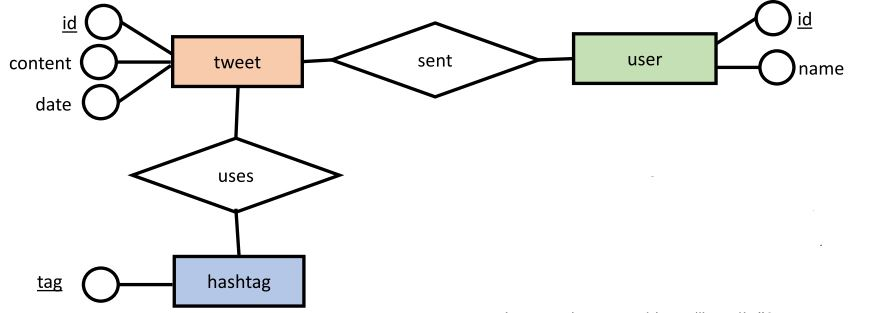
\includegraphics[scale=0.4]{Ex2.JPG}
\end{figure}

%%%%%%%%%%%%%%%%%%%%%%%%%%%%%%%%%%%%%%%%%%%%%%%%%%%%%%%%%%%%%%%%%%%%%%%%%%%%%%%%%%%%%%%%%%%%%%%%%%%%%%%%%%
\subsection{Complex attributes}

\begin{itemize}
    \item \textbf{Computed attributes}: Calculated from other attributes
    \begin{figure} [h!]
        \centering
        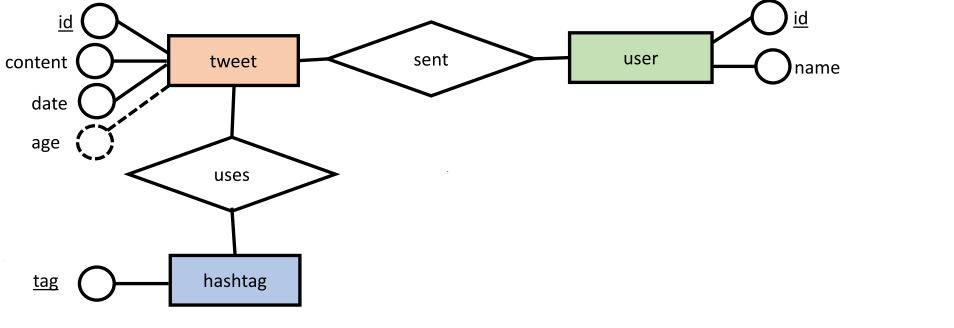
\includegraphics[scale=0.4]{Ex3.JPG}
    \end{figure}
    \item \textbf{Multi-valued attributes}: Sets or lists of multiple values
    \begin{figure} [h!]
        \centering
        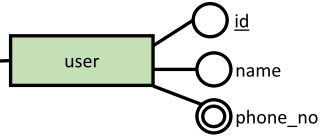
\includegraphics[scale=0.4]{Ex4.JPG}
    \end{figure}
    \item \textbf{Composite attributes}: Properties that has sub-attributes
    \begin{figure} [h!]
        \centering
        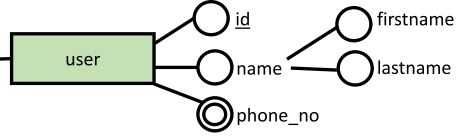
\includegraphics[scale=0.4]{Ex5.JPG}
    \end{figure}
\end{itemize}

\pagebreak

%%%%%%%%%%%%%%%%%%%%%%%%%%%%%%%%%%%%%%%%%%%%%%%%%%%%%%%%%%%%%%%%%%%%%%%%%%%%%%%%%%%%%%%%%%%%%%%%%%%%%%%%%%
\section{Relationships: Sets of relations}

\begin{itemize}
    \item Entity sets contain distinct entities 
    \item \textbf{Relationships} contain sets of relations 
    \item Each \textbf{relation} is a \textit{pair of links} to an entity in the two entity sets
\end{itemize}
\begin{figure} [h!]
    \centering
    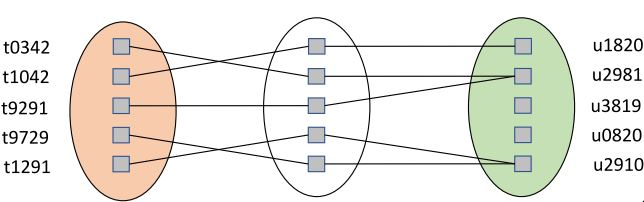
\includegraphics[scale=0.4]{Ex6.JPG}
\end{figure}

%%%%%%%%%%%%%%%%%%%%%%%%%%%%%%%%%%%%%%%%%%%%%%%%%%%%%%%%%%%%%%%%%%%%%%%%%%%%%%%%%%%%%%%%%%%%%%%%%%%%%%%%%%
\subsection{Relation constraints}

\begin{itemize}
    \item \textbf{Cardinality constraint}: Number of times entity appears 
    \begin{itemize}
        \item One-to-one
        \item One-to-many
        \begin{figure} [h!]
            \centering
            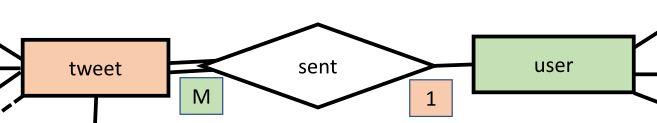
\includegraphics[scale=0.4]{Ex8.JPG}
        \end{figure}
        \item Many-to-many
        \begin{figure} [h!]
            \centering
            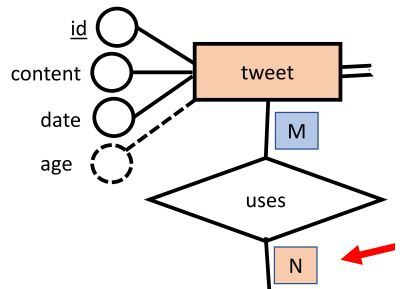
\includegraphics[scale=0.4]{Ex9.JPG}
        \end{figure}
    \end{itemize}
    \item \textbf{Total participation}: Entities \textbf{must} appear in relationships
\end{itemize}
\begin{figure} [h!]
    \centering
    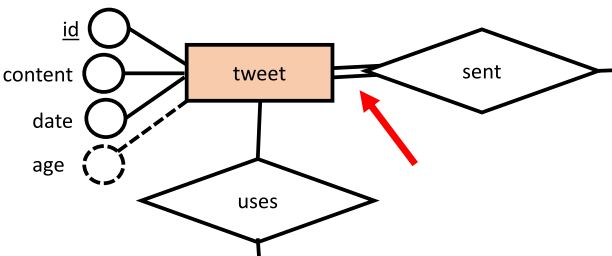
\includegraphics[scale=0.4]{Ex7.JPG}
\end{figure}

%%%%%%%%%%%%%%%%%%%%%%%%%%%%%%%%%%%%%%%%%%%%%%%%%%%%%%%%%%%%%%%%%%%%%%%%%%%%%%%%%%%%%%%%%%%%%%%%%%%%%%%%%%
\subsection{Self relations}

\begin{itemize}
    \item Label the two connecting lines to show \textbf{roles}
    \begin{figure} [h!]
        \centering
        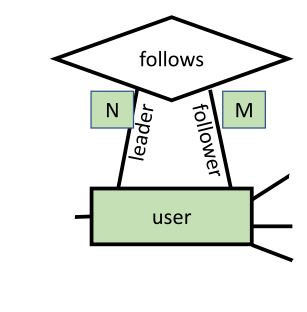
\includegraphics[scale=0.5]{Ex10.JPG}
    \end{figure}

    \item Cardinality constraints still apply
\end{itemize}

%%%%%%%%%%%%%%%%%%%%%%%%%%%%%%%%%%%%%%%%%%%%%%%%%%%%%%%%%%%%%%%%%%%%%%%%%%%%%%%%%%%%%%%%%%%%%%%%%%%%%%%%%%
\subsection{Relations with attributes}

\begin{itemize}
    \item Example: User can like a tweet with emojis
    \begin{figure} [h!]
        \centering
        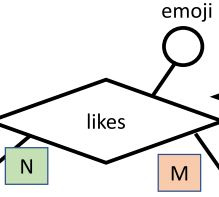
\includegraphics[scale=0.5]{Ex12.JPG}
    \end{figure}
\end{itemize}

\pagebreak

%%%%%%%%%%%%%%%%%%%%%%%%%%%%%%%%%%%%%%%%%%%%%%%%%%%%%%%%%%%%%%%%%%%%%%%%%%%%%%%%%%%%%%%%%%%%%%%%%%%%%%%%%%
\subsection{Three-way relationships}

\begin{itemize}
    \item Some relationships have more than two entity sets
    \item Example: User can \textit{watch} for new retweets
\end{itemize}
\begin{figure} [h!]
    \centering
    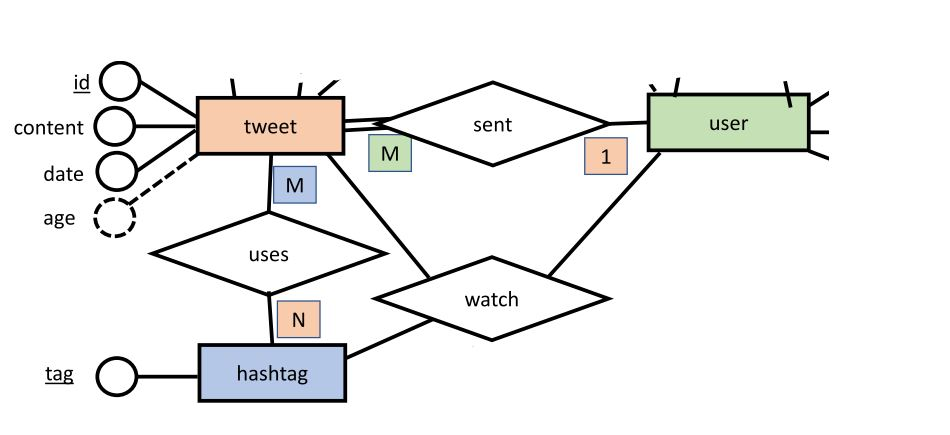
\includegraphics[scale=0.4]{Ex13.JPG}
\end{figure}


%%%%%%%%%%%%%%%%%%%%%%%%%%%%%%%%%%%%%%%%%%%%%%%%%%%%%%%%%%%%%%%%%%%%%%%%%%%%%%%%%%%%%%%%%%%%%%%%%%%%%%%%%%
\end{document}
